% !TeX root = ../../Book2.tex
% 纲要标题：### 3.3 典型空间的整数同调
% 纲要位置：几何学计划纲要.md，第 1135 行。
% 正文状态：初稿；尚未正式审核。

% 纲要内容开始
% 
% * 实射影空间和复射影空间
% * 可定向及不可定向曲面
% * 透镜空间与扭项
% * 附着一个高维胞腔改变什么
% 
% 纲要内容结束

\section{典型空间的整数同调}
\label{g2:sec:0303}

胞腔链群告诉我们各维有多少个待检查的生成元，附着映射才决定哪些生成元成为圈、哪些圈又成为边界。下面的空间都有很少的胞腔，却已经展示了三种不同现象：边界为零时保留自由生成元，非零整数倍的边界产生有限阶同调类，而新增胞腔也可能使原有关系之间出现新的关系。本节的同调均取整数系数。

\subsection{实射影空间和复射影空间}
\label{g2:subsec:0303:01}

\cref{g2:exm:projective-cw}给出的标准分解中，\(\mathbb RP^N\) 在实维数 \(0,1,\ldots,N\) 各有一个胞腔，\(\mathbb CP^N\) 只在实维数 \(0,2,\ldots,2N\) 各有一个胞腔。两个空间都可以用“逐次加入一条新的坐标轴”构造，但它们相邻维数的链群很不相同：实情形允许非零边界，复情形的每一个边界映射都面对一个零群。

\begin{proposition}[射影空间的同调]\label{g2:prop:projective-integer-homology}
	对整数 \(N\geq1\)，实射影空间的整数同调为
	\[
		H_k(\mathbb RP^N)\cong
		\begin{cases}
			\mathbb Z,&k=0,\text{ 或 }k=N\text{ 且 }N\text{ 为奇数},\\
			\mathbb Z/2,&0<k<N\text{ 且 }k\text{ 为奇数},\\
			0,&\text{其余情形}.
		\end{cases}
	\]
	对整数 \(N\geq0\)，复射影空间的整数同调为
	\[
		H_k(\mathbb CP^N)\cong
		\begin{cases}
			\mathbb Z,&k=0,2,\ldots,2N,\\
			0,&\text{其余情形}.
		\end{cases}
	\]
	\(\mathbb RP^0\) 是单点，只有零次同调为 \(\mathbb Z\)。
\end{proposition}
\begin{proof}
	选用\eqref{g2:eq:rp-cellular-boundary}的相容胞腔定向，实射影空间的链复形在 \(0\) 至 \(N\) 次各为 \(\mathbb Z\)，并且
	\[
		\mathrm{d}_k=
		\begin{cases}
			2,&k\text{ 为正偶数},\\
			0,&k\text{ 为奇数}.
		\end{cases}
	\]
	若 \(0<k<N\) 为奇数，所有 \(k\) 链都是圈，而边界是它们的偶数倍，所以 \(H_k=\mathbb Z/2\)；若 \(k>0\) 为偶数，\(\mathrm{d}_k\) 单射，故该次同调为零。最高次须单独看：没有来自 \(N+1\) 次的边界，所以当 \(N\) 为奇数时 \(H_N=\ker\mathrm{d}_N=\mathbb Z\)，不是 \(\mathbb Z/2\)。零次的唯一生成元也没有非零边界。

	在复情形，奇数次链群为零，因此所有胞腔边界均为零，每个偶数次胞腔都给出一个无限阶同调生成元。两种计算通过\cref{g2:thm:cellular-singular-comparison}与奇异同调一致。
\end{proof}

例如，\(\mathbb RP^2\) 的一胞腔本身不是二维胞腔的边界，但它的两倍是边界。这就是 \(\mathbb Z/2\) 所记录的几何事实。对于阿贝尔群 \(G\)，满足 \(ng=0\) 的非零元素 \(g\)（其中 \(n\) 为某个正整数）称为\term[naoyuan]{挠元}[torsion element]；零元与全部挠元组成\term[naoziqun]{挠子群}[torsion subgroup]。本节标题中的“扭项”指这种有限阶信息，它由整数边界系数 \(2\) 保留下来。

\ProseParagraphBreak

无限射影空间要连同拓扑一起说明。令
\[
	\mathbb RP^\infty=\bigcup_{N\geq0}\mathbb RP^N,
	\qquad
	\mathbb CP^\infty=\bigcup_{N\geq0}\mathbb CP^N,
\]
其中包含映射在齐次坐标末尾补零，并赋予上述胞腔分解的弱拓扑。它们的每条胞腔链仍是有限和。由胞腔比较定理，直接使用无限链复形便得到
\[
	H_k(\mathbb RP^\infty)\cong
	\begin{cases}
		\mathbb Z,&k=0,\\
		\mathbb Z/2,&k>0\text{ 为奇数},\\
		0,&k>0\text{ 为偶数},
	\end{cases}
	\qquad
	H_k(\mathbb CP^\infty)\cong
	\begin{cases}
		\mathbb Z,&k\geq0\text{ 为偶数},\\
		0,&k\geq0\text{ 为奇数}.
	\end{cases}
\]
这里没有最高维胞腔，因而没有实射影奇数维顶部的那个例外。若从有限空间理解同一个计算，\cref{g2:thm:finite-subcomplex}保证每条奇异链的紧像落在某个有限子复形中；一个圈成为边界时，其填充链也只用有限多个胞腔。固定次数的结果因此由足够高的有限阶段决定。

\subsection{可定向及不可定向曲面}
\label{g2:subsec:0303:02}

我们使用两类熟悉的闭曲面模型。\(\Sigma_g\) 表示 \(g\) 个环面的连通和，\(g\geq1\)，并令 \(\Sigma_0=S^2\)；\(N_h\) 表示 \(h\) 个实射影平面的连通和，\(h\geq1\)。连通和是从两个曲面各删去一个开圆盘，再将留下的边界圆周粘合。前一类可定向，后一类不可定向；下面的计算只需它们的具体多边形模型。

\ProseParagraphBreak

环面由正方形按边界词 \(aba^{-1}b^{-1}\) 粘合，\(\mathbb RP^2\) 则由圆盘边界的两段按同向的 \(aa\) 粘合。对两个这样的多边形模型作连通和，可以在各自二维胞腔中挖去小圆盘，再切开一条连接内外边界的弧；粘合后，这两条切缝合成一条可重新合起的边，剩余外边界依次读出原来的两个词。因此逐次连通和给出一个顶点、若干条边和一个二维胞腔，其附着词分别为
\begin{equation}\label{g2:eq:surface-attaching-words}
	\Sigma_g:\quad\prod_{i=1}^g a_i b_i a_i^{-1}b_i^{-1},
	\qquad
	N_h:\quad a_1^2a_2^2\cdots a_h^2.
\end{equation}
在这些模型中，每条多边形边都成对粘合；边的内点有圆盘邻域，顶点周围的小扇形也首尾接成一个圆盘。因而商确为无边界曲面。可定向模型的成对边在多边形边界上反向出现，使二维胞腔的定向在粘合处相容；\(a_i^2\) 则在相应闭路周围反转局部定向。

\begin{proposition}[闭曲面模型的同调]\label{g2:prop:surface-integer-homology}
	设 \(\Sigma_g\) 为 \(g\ge0\) 个柄的闭可定向曲面模型（\(\Sigma_0=S^2\)），\(N_h\) 为 \(h\ge1\) 个实射影平面的连通和，取 \eqref{g2:eq:surface-attaching-words} 的胞腔分解。它们的整数同调由下表给出，所有高于二次的同调均为零。
	\begin{center}
		\begin{tabular}{cccc}
			\toprule
			空间 & \(H_0\) & \(H_1\) & \(H_2\)\\
			\midrule
			\(\Sigma_g\)（\(g\geq0\)） & \(\mathbb Z\) & \(\mathbb Z^{2g}\) & \(\mathbb Z\)\\
			\(N_h\)（\(h\geq1\)） & \(\mathbb Z\) & \(\mathbb Z^{h-1}\oplus\mathbb Z/2\) & \(0\)\\
			\bottomrule
		\end{tabular}
	\end{center}
\end{proposition}
\begin{proof}
	先设 \(g\geq1\)。每条边的两端都是唯一的顶点，所以 \(\mathrm{d}_1=0\)。\cref{g2:prop:word-boundary-degrees}把二维胞腔的边界系数化为附着词中各字母的指数和。在 \(\Sigma_g\) 的词中，每个 \(a_i,b_i\) 都以正负指数各出现一次，故 \(\mathrm{d}_2=0\)。其链复形为
	\[
		0\longrightarrow\mathbb Z\xrightarrow{0}\mathbb Z^{2g}
		\xrightarrow{0}\mathbb Z\longrightarrow0,
	\]
	于是得到第一行。\(g=0\) 时用球面的一零胞腔、一二胞腔分解，结论相同。

	在 \(N_h\) 中，每个字母的指数和是 \(2\)，所以
	\[
		\mathrm{d}_2(1)=2(a_1+\cdots+a_h),\qquad\mathrm{d}_1=0.
	\]
	这个 \(\mathrm{d}_2:\mathbb Z\to\mathbb Z^h\) 单射，故 \(H_2=0\)。令 \(v=a_1+\cdots+a_h\)，则 \(v,a_2,\ldots,a_h\) 是 \(\mathbb Z^h\) 的一组整数基，因为 \(a_1=v-a_2-\cdots-a_h\)。在这组基下只剩一个关系 \(2v=0\)，因此
	\[
		H_1(N_h)=\mathbb Z^h/\langle2v\rangle
		\cong\mathbb Z/2\oplus\mathbb Z^{h-1}.
	\]
	两种模型的一维骨架都连通，零次同调为 \(\mathbb Z\)，没有更高维胞腔。
\end{proof}

这里可以看见“边界抵消”与曲面定向的关系。对 \(\Sigma_g\)，二维胞腔的各对边在整数链中互相抵消，整个胞腔成为一个二维圈。对 \(N_h\)，同向出现的边留下系数 \(2\)，不能得到非零二维圈。这些模型中的顶维圈由此直接从多边形边界的符号算出。

\subsection{透镜空间与扭项}
\label{g2:subsec:0303:03}

实射影三维空间的 \(\mathbb Z/2\) 可以推广成任意 \(\mathbb Z/p\)。设 \(p\geq2\)，\(q\in\mathbb Z\) 与 \(p\) 互素，并记 \(\zeta=e^{2\pi\mathrm{i}/p}\)。在
\[
	S^3=\{(z_1,z_2)\in\mathbb C^2:|z_1|^2+|z_2|^2=1\}
\]
上考虑周期变换
\[
	\rho(z_1,z_2)=(\zeta z_1,\zeta^q z_2).
\]
定义三维\term[toujingkongjian]{透镜空间}[lens space]为
\[
	L(p,q)\coloneqq S^3/\langle\rho\rangle.
\]
\symidx{\(L(p,q)\)：三维透镜空间}这里固定的是商作用的参数约定；有些文献改用透镜面上的旋转角作第二参数，得到的公式会出现 \(q\) 的模 \(p\) 逆元。若 \(\rho^j\) 固定一个点，则至少一个坐标非零；由 \(p\mid j\) 或 \(p\mid qj\) 及互素条件，都得到 \(p\mid j\)。因此该作用自由。有限多个不同像可以用互不相交的小邻域分开，所以商投影是 \(p\) 叶覆盖，商空间是闭三维流形。

\begin{figure}[tbp]
	\centering
	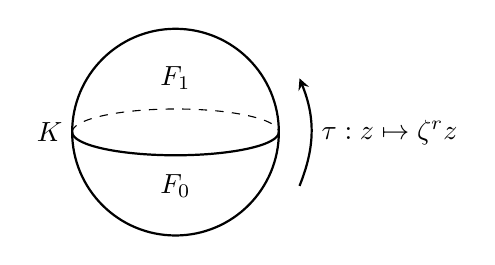
\begin{tikzpicture}[scale=1.05,>=stealth]
		\draw[thick] (0,0) circle (1.25);
		\draw[dashed] (-1.25,0) arc[start angle=180,end angle=0,x radius=1.25,y radius=.28];
		\draw[thick] (-1.25,0) arc[start angle=180,end angle=360,x radius=1.25,y radius=.28];
		\node at (0,.65) {\(F_1\)};
		\node at (0,-.65) {\(F_0\)};
		\node[left] at (-1.25,0) {\(K\)};
		\draw[->,thick] (1.5,-.65) to[bend right=22] node[right] {\(\tau:z\mapsto\zeta^r z\)} (1.5,.65);
	\end{tikzpicture}
	\caption{基本区域三球 \(B\) 的边界示意。两张盘面 \(F_0,F_1\) 沿圆周 \(K\) 相接，并由 \(\tau\) 识别；\(K\) 本身还按 \(p\) 重旋转识别。盘面继承的边界定向相反，边缘的多重绕行则保留在二维边界中。}
	\label{g2:fig:lens-boundary-faces}
\end{figure}

\begin{proposition}[透镜空间的胞腔模型]\label{g2:prop:lens-cellular-model}
	设 \(p\geq2\) 且 \(\gcd(p,q)=1\)。按上述约定定义的 \(L(p,q)\) 有一个在维数 \(0,1,2,3\) 各含一个胞腔的 CW 分解。可以选取胞腔定向，使其整数链复形为
	\begin{equation}\label{g2:eq:lens-cellular-complex}
		0\longrightarrow\mathbb Z\xrightarrow{0}\mathbb Z
		\xrightarrow{p}\mathbb Z\xrightarrow{0}\mathbb Z
		\longrightarrow0.
	\end{equation}
\end{proposition}
\begin{proof}
	我们先找一个基本区域，再读出它的面和边的粘合，\cref{g2:fig:lens-boundary-faces}显示其边界两张盘面的关系。取整数 \(r\) 使 \(rq\equiv1\pmod p\)，并令 \(\tau=\rho^r\)。它仍生成同一个周期群，但在第二坐标上恰旋转 \(2\pi/p\)。在 \(S^3\) 中取扇区
	\[
		B=\left\{\left(z,\sqrt{1-|z|^2}\,e^{\mathrm{i}\theta}\right):
		|z|\leq1,\ 0\leq\theta\leq2\pi/p\right\}.
	\]
	当 \(|z|=1\) 时，第二坐标为零，所有 \(\theta\) 给出同一点。这个集合是闭三球，而不是边界带棱的环面。一个明确的参数说明如下：从普通闭三球 \(\{(z,s):|z|^2+s^2\leq1\}\subset\mathbb C\times\mathbb R\) 出发，在 \(|z|<1\) 时令
	\[
		\theta=\frac{\pi}{p}\left(1+\frac{s}{\sqrt{1-|z|^2}}\right),
	\]
	再代入 \(B\) 的公式；在 \(|z|=1\) 时取 \((z,0)\)。因为趋近边缘时第二坐标的模趋于零，该映射连续；它是紧空间到 Hausdorff 空间的连续双射，故是同胚。

	三球边界分成两个闭圆盘
	\[
		F_j=\left\{\left(z,\sqrt{1-|z|^2}\,e^{2\pi\mathrm{i}j/p}\right):|z|\leq1\right\},
		\qquad j=0,1,
	\]
	它们沿公共圆周 \(K=\{(z,0):|z|=1\}\) 相交。\(\tau\) 把 \(F_0\) 送到 \(F_1\)，在盘坐标中是旋转 \(z\mapsto\zeta^r z\)。若 \(z_2\ne0\) 且其辐角不是 \(2\pi/p\) 的整数倍，该轨道在扇区内部恰有一个代表；若辐角为 \(2\pi/p\) 的整数倍，则在两个盘面内部各有一个代表，它们由上述面粘合识别。剩下的点都位于 \(K\)，其识别为 \(z\sim\zeta z\)。因此从 \(B\) 出发作这些识别，恰得到 \(L(p,q)\)。

	边缘商 \(K/\langle\zeta\rangle\) 是圆周，商坐标可取 \(z\mapsto z^p\)，给它选一个顶点和一条开边。盘面内部的公共像是一开二胞腔，\(B\) 的内部是一开三胞腔；其余点都在刚才的圆周内。这给出所述四个胞腔。它们的特征映射来自圆盘和三球到商空间的映射；空间紧且只有有限多个胞腔，因此附着拓扑与所得商拓扑一致。

	给二胞腔选取 \(F_0\) 的复平面定向，其边界绕 \(K\) 一周；在商圆周中则由 \(z\mapsto z^p\) 绕行 \(p\) 周。因此\cref{g2:thm:cellular-boundary-degree}给出 \(\mathrm{d}_2=p\)。唯一一胞腔的两端相同，故 \(\mathrm{d}_1=0\)。

	最后计算 \(\mathrm{d}_3\)。把三球边界的两个半球都用同一个盘坐标 \(z\) 表示时，它们从三球继承的边界定向相反。两面的识别 \(z\mapsto\zeta^r z\) 又保持盘定向。在二胞腔内部取一点，它在这两个面中各有一个原像，局部度一正一负；压掉一维骨架以后，其度之和为 \(1-1=0\)。这就是 \(\mathrm{d}_3=0\) 的来源。
\end{proof}

两个盘面的定向抵消只说明三胞腔的边界系数为零；二胞腔边缘上的 \(p\) 重绕行仍然存在。由\eqref{g2:eq:lens-cellular-complex}立即得到
\begin{equation}\label{g2:eq:lens-integer-homology}
	H_k(L(p,q))\cong
	\begin{cases}
		\mathbb Z,&k=0,3,\\
		\mathbb Z/p,&k=1,\\
		0,&\text{其余情形}.
	\end{cases}
\end{equation}
一胞腔给出的圈有阶恰为 \(p\)：它的 \(p\) 倍被二胞腔填充，任何较小正倍数都不在 \(p\mathbb Z\) 内。这一计算保留了覆盖重数 \(p\)，却没有保留盘面旋转中的全部参数 \(q\)；因此相同的这组同调群本身不能回答两个透镜空间是否同胚。特别地，\(L(2,1)=\mathbb RP^3\)，与前面的结果吻合。上述胞腔模型也可对照\cite[第2.2节，Cellular Homology]{Hatcher2002}。

\subsection{附着一个高维胞腔改变什么}
\label{g2:subsec:0303:04}

附着球面在旧空间中的同调类，可以是无限阶、有限阶或零。空间对的长正合列分别给出这三种情形中新生成的类与新施加的关系，并说明一次附着只可能影响两个相邻次数的同调。

\begin{proposition}[单胞腔附着的同调变化]\label{g2:prop:single-cell-homology-change}
	设 \(X\) 是非空 CW 复形，\(m\geq2\)，\(\alpha:S^{m-1}\to X^{m-1}\) 连续，并令 \(Y=X\cup_\alpha D^m\)。给圆盘选定向，球面取相应边界定向，记 \(u=\alpha_*[S^{m-1}]\in H_{m-1}(X)\)。则包含 \(X\hookrightarrow Y\) 在 \(k\notin\{m,m-1\}\) 时诱导同构 \(H_k(X)\cong H_k(Y)\)，且有正合列
	\begin{equation}\label{g2:eq:single-cell-six-term}
		\begin{gathered}
			0\longrightarrow H_m(X)\longrightarrow H_m(Y)\longrightarrow\mathbb Z\\
			\xrightarrow{\,1\mapsto u\,}H_{m-1}(X)\longrightarrow H_{m-1}(Y)\longrightarrow0.
		\end{gathered}
	\end{equation}
	特别地，\(H_{m-1}(Y)\cong H_{m-1}(X)/\langle u\rangle\)。若 \(u\) 为无限阶，则 \(H_m(Y)\cong H_m(X)\)；若 \(u\) 有有限阶（包括 \(u=0\)），则存在群同构 \(H_m(Y)\cong H_m(X)\oplus\mathbb Z\)，但后一分解一般没有指定的自然选择。
\end{proposition}
\begin{proof}
	相对胞腔复形 \(C^{\mathrm{cell}}_\bullet(Y,X)\) 只剩新增的一个 \(m\) 次生成元，所有微分为零。由\cref{g2:thm:relative-cellular-comparison}，相对奇异同调为
	\[
		H_k(Y,X)\cong
		\begin{cases}
			\mathbb Z,&k=m,\\
			0,&k\ne m.
		\end{cases}
	\]
	代入\cref{g2:thm:pair-LES}便得到不受影响的次数和\eqref{g2:eq:single-cell-six-term}。还要认清其中的连接同态：特征映射是空间对映射 \((D^m,S^{m-1})\to(Y,X)\)，其相对定向类给出上面 \(\mathbb Z\) 的生成元。连接同态的自然性，以及“取代表链的边界”这一约定，说明它的像恰为 \(\alpha_*[S^{m-1}]=u\)。

	由正合性，低一次群是所述商群，而最高一段可以写成
	\[
		0\longrightarrow H_m(X)\longrightarrow H_m(Y)
		\longrightarrow K\longrightarrow0,
		\qquad K=\{a\in\mathbb Z:au=0\}.
	\]
	若 \(u\) 为无限阶，则 \(K=0\)。若 \(u\) 的阶为 \(s<\infty\)，约定零元的阶为 \(1\)，则 \(K=s\mathbb Z\cong\mathbb Z\)。在 \(H_m(Y)\) 中选一个映到 \(s\) 的元素，它的整数倍给出该短正合列的分裂，因而得到直和分解。更换这个提升可以加上 \(H_m(X)\) 中的元素，所以分解不由原数据唯一指定。
\end{proof}

若 \(u\ne0\) 的阶为 \(s\)，新增胞腔本身的边界还没有消失，但它的 \(s\) 倍的边界能在 \(X\) 中填充。用 \(s\) 份新胞腔减去这条旧填充链，才得到一个新的 \(m\) 维圈。于是一次附着可以同时消去低一次的挠类，并产生高一次的无限阶类。

\begin{example}[在球面上附着一个胞腔]\label{g2:exm:degree-cell-attachment}
	设 \(m\geq2\)，\(f:S^{m-1}\to S^{m-1}\) 的度为 \(a\in\mathbb Z\)，并令 \(Y=S^{m-1}\cup_fD^m\)。取球面的一零胞腔、一 \((m-1)\) 胞腔分解，则其唯一可能非零的高次边界为 \(\mathrm{d}_m=a\)。若 \(a\ne0\)，则
	\[
		\widetilde H_{m-1}(Y)=\mathbb Z/a\mathbb Z,
		\qquad \widetilde H_k(Y)=0\quad(k\ne m-1).
	\]
	若 \(a=0\)，则 \(\widetilde H_m(Y)=\widetilde H_{m-1}(Y)=\mathbb Z\)，其余约化同调为零。这也可逐项代入\eqref{g2:eq:single-cell-six-term}得到。对于 \(|a|=1\)，附着后约化同调全部消失；对于 \(|a|>1\)，留下阶为 \(|a|\) 的类。同调计算本身没有进一步证明这个空间在前一种情形可缩，也没有把后一种情形的整个同伦型归结为这些群。
\end{example}

这些例子把胞腔数、附着的整数系数和最终同调分开了。胞腔数相同可以有不同的同调；同调相同也只表示这里计算的阿贝尔群信息相同。要可靠地处理胞腔较多的空间，还需在整数基中同时控制核与像，这正是下一节边界矩阵计算的任务。
% 纲要条目排为编号小节标题，并进入目录与书签；说明段仍保留于纲要注释中。
